\documentclass[]{rs}

%%%========= 基本信息 =========%%%

\mytitle{《Latex编程基础课程实习》\\实习报告}
\Ccollege{遥感信息工程学院}
\Cclass{21XX}
\CstudentNum{2021302131XXX}
\Cname{QHD}
\Cplace{宿舍}
\Cteacher{CSDN,ChatGPT}
\Cdate{2024年5月22日}

%%%========= Begin Doc =========%%%

\begin{document}

%%%========= 封面 =========%%%

\maketitle

%%%========= 目录 =========%%%

\centering{\tableofcontents}
\thispagestyle{empty} % 目录页没有页脚
\newpage
\setcounter{page}{1} % 刷新页数,从正文开始计数

%%%========= 正文 =========%%%

\section{模板介绍}

根据武汉大学遥感信息工程学院课程实习Word模板排版而成的Latex模板。

\section{文件目录说明}

- content/ 放置正文

- figure/ 放置图片

- main.tex 主文件(在这里修改基本信息)

- refs.bib 参考文献

- rs.cls Latex样式文件(不要轻易改动,除非知道自己在做什么)

\section{参考文献的使用}

使用cite语句链接bib文件中的参考文献。\cite{CMJH200711001007}

\section{图片的使用}

\begin{figure}[H]% 插入一张图片,H表示浮动环境下的here
    \centering
    \begin{minipage}{0.83\textwidth}% 小页面尺寸,可自行调节
        \centering
        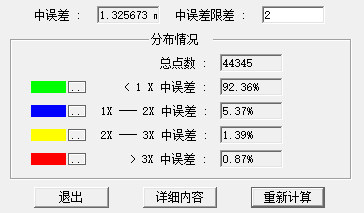
\includegraphics[width=1.0% 图片尺寸,可自行调节
        \textwidth]{figure/DEM拼接精度.png}% 
        \caption{\fontsize{10pt}{15pt}\selectfont 示例图片}
    \end{minipage}
\end{figure}

\section{并排的两张图片}

\begin{figure}[H]
        \setcounter{0}
	\subfigure%多张图片
	{
		\begin{minipage}[b]{.5\linewidth}%小页占行宽0.5
			\centering
			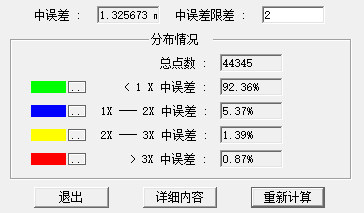
\includegraphics[scale=0.5]{figure/DEM拼接精度.png}
            \caption{示例图片1}
            \label{示例图片1}
		\end{minipage}
	}  %可以试加空格排版合适,不然可能重合(一般调整小页大小就可以了
        \setcounter{0}
	\subfigure
	{
		\begin{minipage}[b]{.5\linewidth}
  \centering
	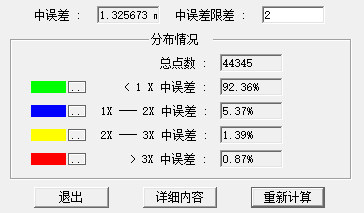
\includegraphics[scale=0.5]{figure/DEM拼接精度.png}
            \caption{示例图片2}
            \label{示例图片2}
		\end{minipage}
	}
 \end{figure}

\section{三线表的使用}

\begin{table}[H]
    \centering
    \caption{双对数需求模型回归结果}
    \label{table_gk}
        \begin{tabular}{c|cccccc}%没有竖直竖线
        \toprule[1.5pt]%最上方横线
        \makebox[0.06\textwidth][c]{}	& \makebox[0.1\textwidth][c]{lnQ1}	& \makebox[0.1\textwidth][c]{lnQ2}	& \makebox[0.1\textwidth][c]{lnQ3}	& \makebox[0.1\textwidth][c]{lnQ4}	& \makebox[0.1\textwidth][c]{lnQ5}	& \makebox[0.1\textwidth][c]{lnQ6}	   \\ \hline
        lnP1   & -0.186*** & -0.08***  & -0.058*** & 0.035***  & -0.103*** & -0.088*** \\
        lnP2   & 0.044     & -0.076*** & -0.241*** & -0.397*** & -0.661*** & -0.032    \\
        lnP3   & 0.03**    & -0.217*** & -0.221*** & -0.074***  & -0.108**  & -0.012    \\
        lnP4   & 0.193***  & 0         & -0.075*** & -0.168*** & -0.072*** & -0.07***  \\
        lnP5   & -0.007    & -0.159*** & -0.036**  & 0.139***  & -0.43***  & -0.272*** \\
        lnP6   & 0.023     & -0.433*** & -0.078*** & -0.142*** & -0.042*** & -0.381*** \\
        PQ     & -0.032    & 0.956***  & 0.678***  & 0.605*** & 1..441*** & 0.951***  \\ \hline
        F显著性水平 & ***       & ***       & ***       & ***       & ***       & ***    \\
        \bottomrule[1.5pt]%最底下横线
        \end{tabular}
        \begin{tabular}{p{0.9\textwidth}}
        \textit{1、***、** 分别表示 1\%,5\% 的显著性水平}\\
        \textit{2、1 至 6 分别为:水生根茎类、花叶类、花菜类、茄类、辣椒类、食用菌}
        \end{tabular}
\end{table}

\section{公式的使用}

\begin{equation}
Q_j=v\frac{S_j-S^*}{S^--S^*}+(1-v)\frac{R_j-R^*}{R^--R^*},i=1,2,\cdots,m
\end{equation}


\section{插入代码块}

\addcode{python}{code/test.py}



% 可以根据上述格式添加多个正文文件
% 示例:
% >>> \input{content/text1}
% >>> \input{content/text2}
% >>> \input{content/text3}

%%%========= 参考文献 =========%%%
% 不想要参考文献可以直接把这部分注释掉

\phantomsection\addcontentsline{toc}{section}{参考文献}\tolerance=500 %将参考文献放进目录
\cleardoublepage\phantomsection
\bibliographystyle{gbt7714-numerical}
\bibliography{refs.bib}

%%%========= End Doc =========%%%
\end{document}


